\documentclass[15pt]{article}
\usepackage{graphicx,fullpage,blindtext,amsmath,amssymb,listings,pgfplots,pgfplotstable}
\graphicspath{ {images/} }
\usepackage[utf8]{inputenc}
\usepackage[absolute]{textpos}
\setlength{\TPHorizModule}{1cm}
\setlength{\TPVertModule}{1cm}
\pgfplotsset{compat=1.7}
\usepackage{tikz}
\title{\emph{2020-2021\\Game Theory and Its Applications\\CS 9042}}
\author{
Arghya Bandyopadhyay
}
\date{27th March 2021}
\begin{document}
\begin{textblock}{5}(14,1)
\noindent\Large \[\frac{M.Tech./Even/2020-21}{\textbf{\emph{Mid-Term(2nd Assessment)}}}\]
\end{textblock}
\maketitle
\begin{enumerate}
\item
\begin{enumerate}
\item

Say there is a dictator voter in a system. What is the implication
of that? In this context state two theorems that has been very
fundamental to the voting theory. Explain the effectiveness of the
two theorems with examples.
\begin{flushright}
[1+2+2] (CO2)
\end{flushright}
\textbf{\emph{Answer: }}The implications of the dictator voter in a system states that for a dictator voter i, the dictator rule elects i's first choice.\\
The two theorm that has been very fundamental to this voting theory are\\

\begin{enumerate}
\item Gibbard-Satterthwaite theorm:- It states that wvery strategyproof voting rule that can produce atleast three different outcomes is a dictator.
\item Arrow's impossibility theorm:- It states that, with three or more alternatives, no voting rule satisfies the following three properties:
\begin{itemize}
\item Non-dictatorship
\item Unanimity
\item Independent of irrelevant alternatives
\end{itemize}
\end{enumerate}

Non dictatorship means that there is no dictators in the system. Unanimity means that in case every voter ranks a over b, then the voting rule should also rank a over b. And, IIA implies that for every pair a,b of alternatives, the relative order of a,b in the produced ranking should be a function only of the relative order of a,b in each voters list, and not depend on the position of irrelevant alternatives.

For example, the plurality rule doesnot satisfy IIA; the outcome of 2000 U.S. Presidential election was certainly not independent of the position of Nader in voter's preference list. More generally, a voting rule that allows spoiler candidate cannot satisfy IIA.\\

\item Say there is a site and in that site very few people upload and
bulk of the people just enjoy downloading. What will happen for
the site in the long run? Explain the phenomena with repeated
games.
\begin{flushright}
[5] (CO1, CO3)
\end{flushright}
\textbf{\emph{Answer: }}According to the question, there is a site where there are very few people who upload whereas there are bulk of people who just enjoy downloading.\\

As a result of which, cost of defect will increase as compared to cost of cooperation.\\
In long term if this continues then the game might stop.\\
Let us take a look at an individual person, he/she has two choices,
\begin{enumerate}
\item upload
\item Dont upload
\end{enumerate}

What was the individual best response, it was don't upload that was the dominant strategy solution for the game i.e when the game is been played between users.
So, a prisoner's dilemma situation is happening \& we can say that because of this, many people had a free ride(don't upload in this case)
However, there are some people, who are uploading the files \& restore downloading the game is being played in a repeated manner.

But in subsequent years the site will slowly approach towards extinction.\\
\item Write an algorithm for the ranked choice voting in a pseudocode
form. With an example explain its salient features.
\begin{flushright}
[3] (CO2)
\end{flushright}
\textbf{\emph{Answer: }}\\ \textbf{Ranked-Choice voting:-}
\begin{enumerate}
\item Voters submit a full ranked list
\item If there is some alternatives a* that received more than 50\% of the first choice votes,
then, a* is the winner
\item Else, the alternative with the fewest first-choice votes is deleted \& the winner is computed recursively on the remaining alternatives.
\end{enumerate}
Ranked choice voting is not strategyproof. The intuition is that there can be an incentive to influence who gets eliminated early on, so that our preffered guy gets more favoured matchups in later rounds. Compared to the plurality rule, however it seems trickier for a voter to reason about how to game the system in ranked choice voiting. This is one of the reason why most voting to plurality voting.
For example, even if we know everyone else's votes, the problem of checking for a profitable manipulation is NP Hard.\\
\end{enumerate}
\item
\begin{enumerate}
\item Say there is a long road and throughout the road several houses
are there. Now say, the town authority wants to open a medical
unit some where beside the road. You cast this problem as a vot-
ing problem and provide a strategyproof and a non-strategyproof
voting rule for this. Illustrate your idea with examples.
\begin{flushright}
[1+3+2] (CO2)
\end{flushright}
\textbf{\emph{Answer: }} Suppose each voter votes by providing a reported peak. \[x_i\epsilon [0,1]\] Which alternative should we choose?
One can imagine scenarios where single peaked preference are a reasonable first cut approx of voter's preference. i.e Selecting a point for medical hospital.
One idea is to choose the average, \[\frac{1}{n} \sum_{i=1}^{n} x_i\] But note that this is not strategyproof. A voter might be able to pull the chosen outcome closer to her peak by reporting an overly extreme peak. A second \& better idea is to choose the median of the reported peaks. The median voting rule is strategyproof. The only way a voter can manipulate the median is to report a peak on the opposite side of the median from her true peak. But this can only pull the median far away from her true peak, a worse outcome for her.
\begin{center}
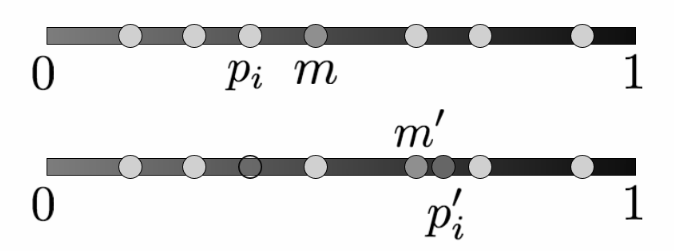
\includegraphics[width=0.42\textwidth]{graph.png}\\
\end{center}
Figure- Median m of reported peaks(with n=7). A voter i with peak $p_i$ cannot change the median unless she overshoots to other side by misreporting $p_i'$ this would move median $ m' $ further.\\
\item Explain Nash equilibrium in the context of the routing game. Explain with examples.
\begin{flushright}
[3](CO2)
\end{flushright}
\textbf{\emph{Answer: }}\\ \textbf{Nash Equilibrium:-}
\begin{enumerate}
\item It is a concept within game theory where the optimal outcome of a game is where there is no incentive to deviate from the initial strategy.
\item More specifically, the Nash equilibrium is a concept of game theory, where no player has an incentive to deviate from their chosen strategy after considering an opponent's choice.
\item \textbf{For Example:} If two players Alice \& Bob choose strategy A \& B, (A,B) is a Nash Equilibrium. If Alice has no other strategy available that does better than A, at maximizing her payoff in response to Bob choosing B and B has no other strategy available that does better than B at maximizing his payoff in response to Alice choosing A.
\end{enumerate}
\item Say there is a matrimony site. How game theoretic concept may
be applied for that site. Illustrate with examples.
\begin{flushright}
[3] (CO1 and CO2)
\end{flushright}
\textbf{\emph{Answer: }} In a matrimonial site, a game theory concept for marraige is the stable matching theorm (Gale shapley Algorithm)
In this, the matching is generally a projection from one set of elements to other sets.
\begin{enumerate}
\item There is an element A of first matched set which prefer some given element B of second matched set over to element A which is already matched.
\item B also prefers A over the element to which B is already matched.
\end{enumerate}
\textbf{For Example}, Let there be 3 men A,B,C \& 3 women D,E,F the preference by each of them are\\
\begin{center}
\begin{tabular}{ |c|c c c| } 
 \hline
 A & E & F & D \\ [0.5ex] 
 \hline
 B & D & E & F \\ 
 \hline
 C & F & D & E \\ [1ex] 
 \hline
\end{tabular}
\begin{tabular}{ |c|c c c| } 
 \hline
 D & A & C & B \\ [0.5ex] 
 \hline
 E & C & B & A \\ 
 \hline
 F & B & A & C \\ [1ex] 
 \hline
\end{tabular}
\end{center}
A has E as its first preference \& E has A as its last but C \& B haven't opted for E $\therefore$ A \& E are being matched. So in this way stable marraige$/$ stable matching is being done at the matrimonial site.
\end{enumerate}
\end{enumerate}
\end{document}
